\section{Placement Results}
\label{sec:results}


We will need an HDL design that utilizes a good mixture of LUTs, FFs, BRAMs, and DSPs at scale to demonstrate the robustness and performance of our placers. 
Any DSP subsystem can serve as a good candidate for such a demonstration. 
Here, we will perform placement on a 2048-order FIR Filter which was conveniently created as coursework for a VLSI course. 
After passing synthesis, the FIR Filter design calls for the primitive cells shown in the second column of table \ref{fig:utilization}.
We will perform placement of this design on a \texttt{xc7z020} FPGA, which is a mid-ranged Xilinx device containing the available BELs shown in the first column of table \ref{fig:utilization}.
Note that \texttt{LUT5-LUT6} pairs are counted as a single \texttt{LUT}.
% Also note that the number of \texttt{CARRY4} BELs is equal to the total number of \texttt{SLICEL} and \texttt{SLICEM} Sites combined and that the number of \texttt{LUT}s is equal to four times that amount while the number of \texttt{FF}s is equal to eight times that amount.

\vspace{0.25cm}
{
    \centering
    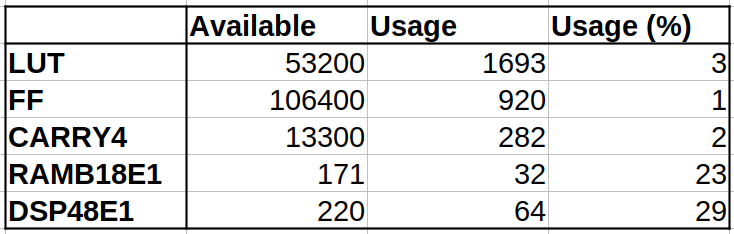
\includegraphics[width=0.8\columnwidth]{figures/results/utilization.png}
    \captionof{figure}{Utilization of BELs on a \texttt{xc7z020} FPGA for a FIR filter design}
    \label{fig:utilization}
}
\vspace{0.25cm}

Now, we present test results for a basic SA placer as well as test results for four simple variations as listed below. 
Note that midpoint simply means centroid.

\begin{itemize}
    \item \texttt{PlacerGreedyRandom}: all undirected random moves with greedy acceptance
    \item \texttt{PlacerGreedyMidpoint}: all directed centroid moves with greedy acceptance
    \item \texttt{PlacerAnnealRandom}: all undirected random moves with annealing acceptance \textbf{(the basic SA algorithm)}
    \item \texttt{PlacerAnnealMidpoint}: all directed centroid moves with annealing acceptance
    \item \texttt{PlacerAnnealHybrid}: \textbf{Initial:} 50\% random - 50\% centroid moves with annealing acceptance. \textbf{At Near-Zero Temperature:} 100\% centroid moves with annealing acceptance.
\end{itemize}

Shown in figure \ref{fig:placers_overlay} are the HPWL curves for each of the five placers. 
\texttt{PlacerGreedyMidpoint} (in red) appears to perform the worst by a considerable margin with a final HPWL cost of 590K.
This is likely due to the lack of randomness or lack of diversity in move proposals combined with the persistent greediness of the movement acceptance that prevents the system from escaping local minima.
This conclusion is supported by its HPWL curve (in red) showing a sharp drop in cost that quickly asymptotes just below the 600K mark, suggesting that the system crystallized very quickly into a local minimum and was unable to climb out of it.

Next is \texttt{PlacerAnnealMidpoint} with a final cost of 466K.
Like the previous placer, \texttt{PlacerAnnealMidpoint} lacks the diversity of random moves which contributes to faster crystallization into local minima.
However, this placer likely performed better than the previous as there is still some randomness in the move acceptance evaluation which gives way to occasional hill-climbing. 
Keep in mind that centroid moves do not necessarily decrease system cost. 
The centroid move can decrease the HPWL cost of the nets on connected to the current \texttt{SiteInst}, but can potentially increase the cost of another group of nets in the event of a swap, which can potentially result in an increase in total system cost.

The next three placers performed better than the previous two placers by decent margin.
The vanilla SA placer, \texttt{PlacerAnnealRandom}, is represented by the green curve.
We can observe that the cost decreases more steadily than the previous two placers, with noticeable spikes in total system cost due to hill-climbing, until settling at the 346K mark as the global temperature cools to zero.

Next is \texttt{PlacerGreedyRandom} which is represented by the purple curve.
We can observe a much steeper initial drop in system cost than the vanilla SA placer due to greedy movement acceptance.
Interestingly, this placer also settled at a lower final system cost of 333K, which is a slight 4\% improvement over vanilla SA.
We originally expected the greediness to be a detriment to finding the global minimum, but due to the inherent randomness of the algorithm, these broader trends will require many more test trials to reliably observe.

{
    \centering
    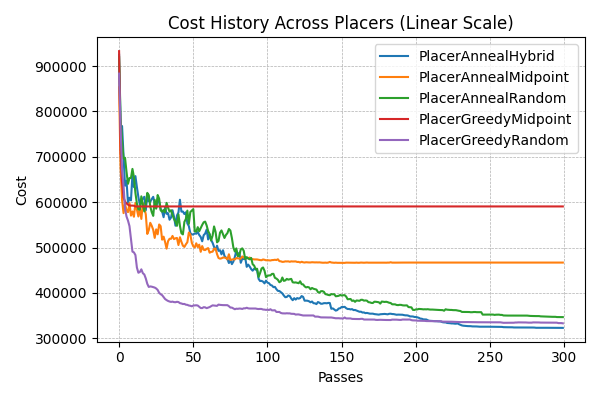
\includegraphics[width=\columnwidth]{figures/results/combined_cost_history_linear.png}
    \captionof{figure}{All placers overlaid}
    \label{fig:placers_overlay}
}

The best performing placer was \texttt{PlacerAnnealHybrid}, represented by the blue curve.
Starting at zero passes, the placer randomly selects between random selection and centroid selection, allowing the placer to make on average more cost-reducing moves, while still maintaining some diversity of moves for hill-climbing. 
Then, at near-zero temperature, the placer makes exclusively centroid moves with annealing acceptance to speed up the final crystallization into the local minimum. 
With centroid moves and annealing acceptance, hill-climbing can only be achieved via swaps.
We can observe that \texttt{AnnealHybrid} settles at a similar rate with the vanilla \texttt{AnnealRandom}, but eventually settles at a lower minimum at 322K, slightly outperforming \texttt{GreedyRandom}. 

{
    \centering
    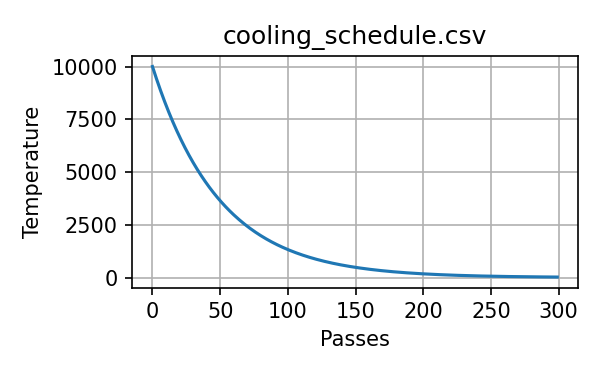
\includegraphics[width=0.6\columnwidth]{figures/placement/cooling_schedule_10000_98.png}
    \captionof{figure}{Cooling Schedule: \(T_0=10000\), \(\alpha=0.98\)}
    \label{fig:cooling_schedule_10000_98}
}
\vspace{1.0cm}

Figures \ref{fig:PGRSnapshots}, \ref{fig:PGMSnapshots}, \ref{fig:PARSnapshots}, \ref{fig:PAMSnapshots}, and \ref{fig:PAHSnapshots} show snapshots of the placement progress on the physical \texttt{device} after 0, 10, 100, and 300 passes for each placer variant.

Please zoom into the document to render the figures in greater detail.
All black areas represent purely routing \texttt{Site}s that contain no logic resources. 
All gray or dull-colored boxes represent \texttt{Site}s that are unoccupied by \texttt{SiteInst}s, while brightly filled boxes represent \texttt{Site}s that are occupied by the supported library of \texttt{SiteInst}s.
Cyan boxes represent occupied \texttt{SLICEL}s, magenta boxes represent occupied \texttt{RAMB18E1}s, and yellow boxes represent occupied \texttt{DSP48E1}s.

The tangle of red lines represent the nets between the \texttt{Site}s, which are yet to be routed at this stage. 
Brighter red lines represent nets of higher total HPWL, while duller red lines represent nets of lower total HPWL.
Notice there are two brightly red nets in every figure that have a particularly high fanout:
one sourced from the near-center, and another sourced from the top right of the device. 

The singular white box in the near-center of all of the figures represents an occupied \texttt{BUFGCTRL} \texttt{Site}, which is a clock buffer used to route clock nets. 
Since clock nets tend to have very high fanout, they can use up an unnecessarily large portion of routing resources if they are routed through general routing.
Modern FPGAs like the 7-Series have dedicated clock tree routes which can evenly distribute clock signals to all logical \texttt{Site}s without burdening the general routing resources.
These special clock routes are accessed by routing the raw clock signal from the crystal oscillator IO port to one these on-chip clock buffers which connects to the on-chip clock tree network.
It is always best practice to use them to improve the routability of the design, and simultaneously, to reduce clock skew and improve timing. 
Our simple FIR Filter design only operates on a single clock domain, so only one clock buffer \texttt{Site} is used. 
An HDL design operating on many clock domains will use more clock buffers or a dedicated clock generator such as a phase locked loop (PLL) or mixed-mode clock manager (MCMM).

The right and left edges of the FPGA device is where most of the general purpose I/O (GPIO) is located. 
In the top right of the device is where we source our reset signal. 
Like the clock net, the reset net also has high fanout and is supplied to all synchronous elements.
Unlike clock signals, reset signals are not subject to sensitive timing constraints as they are not active on most clock cycles and can tolerate higher skew.
Thus, they are simply routed via general routing.

Observe how \texttt{PlacerGreedyMidpoint} \ref{fig:PGMSnapshots} and \texttt{PlacerAnnealMidpoint} \ref{fig:PAMSnapshots} both show almost not shrinkage in profile after the first 10 iterations, likely owing to the inability to hill-climb, while the other three placers show incremental shrinkage.

Also note the sparsity of the \texttt{DSP48E1} (yellow) and \texttt{RAMB18E1} (magenta) \texttt{Site} columns compared to the more uniform grid of \texttt{SLICEL}s (cyan), which poses a computational challenge for the legalization process in directed and analytical placement.


\newpage
\end{multicols}
{
    \centering
    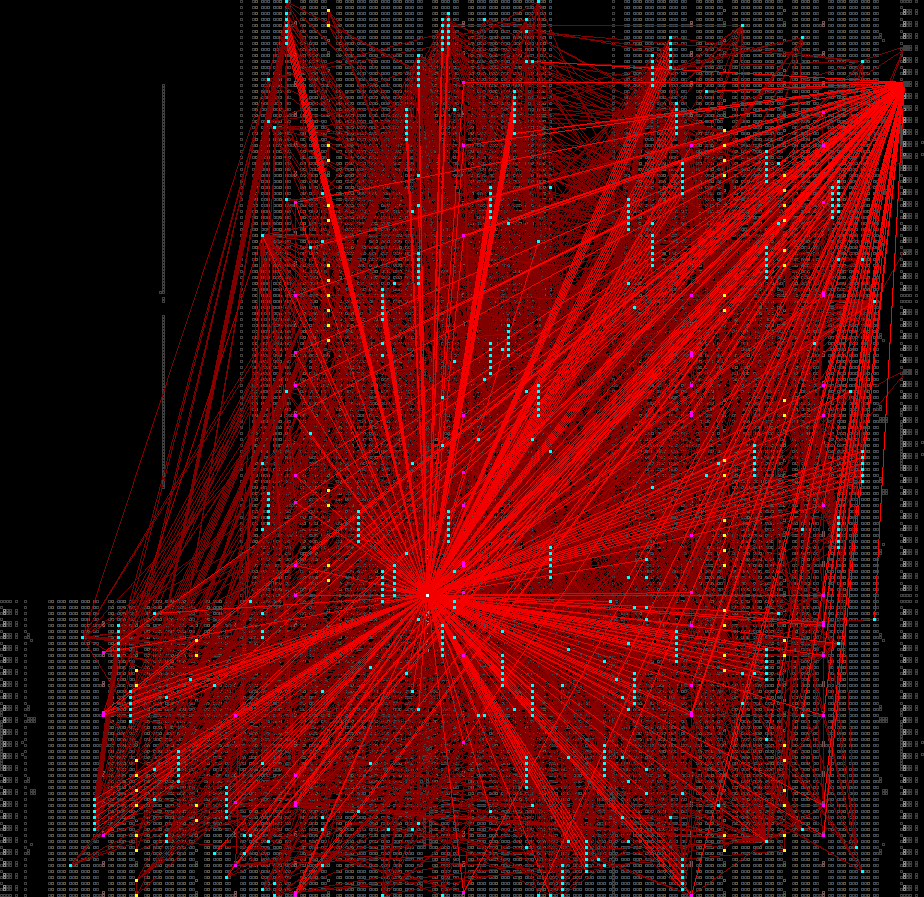
\includegraphics[valign=t, scale=0.13]{figures/results/PlacerGreedyRandom/random_placement.png}
    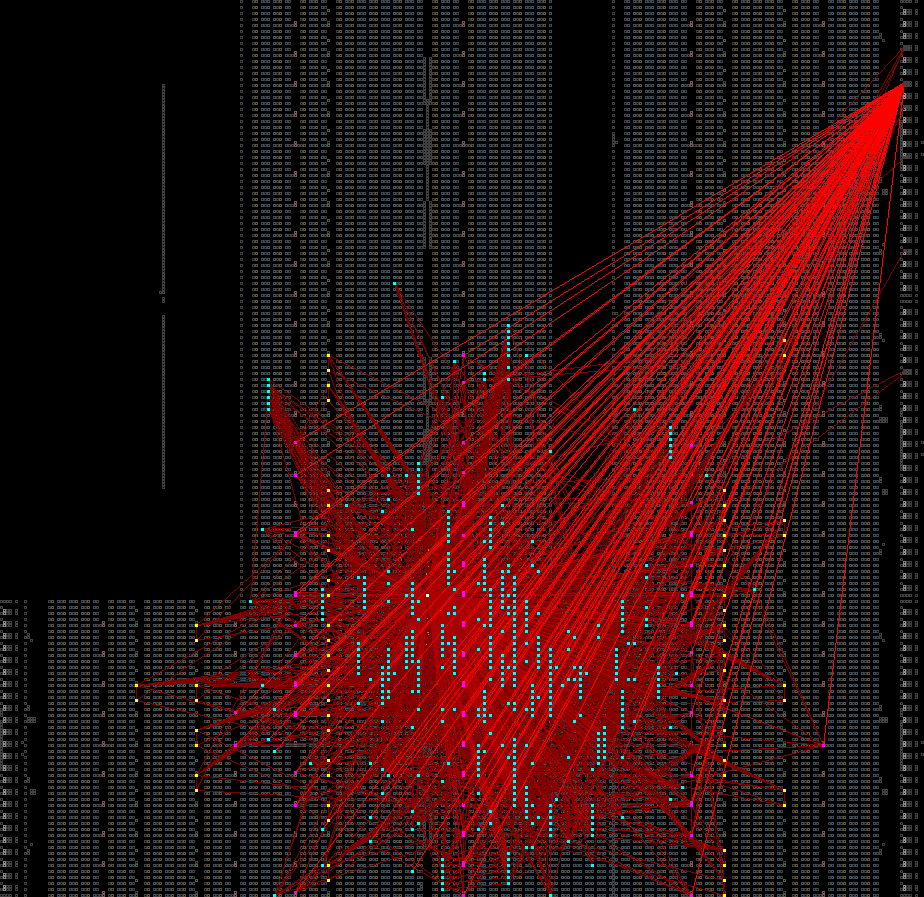
\includegraphics[valign=t, scale=0.13]{figures/results/PlacerGreedyRandom/00000010.png}
    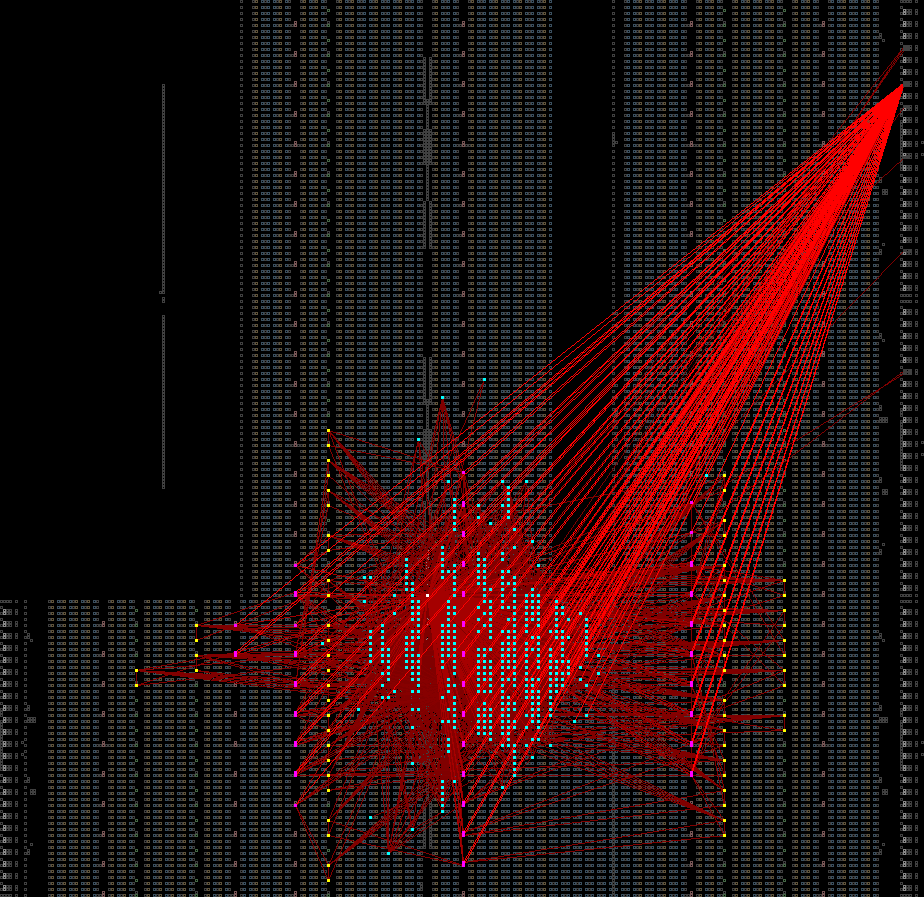
\includegraphics[valign=t, scale=0.13]{figures/results/PlacerGreedyRandom/00000100.png}
    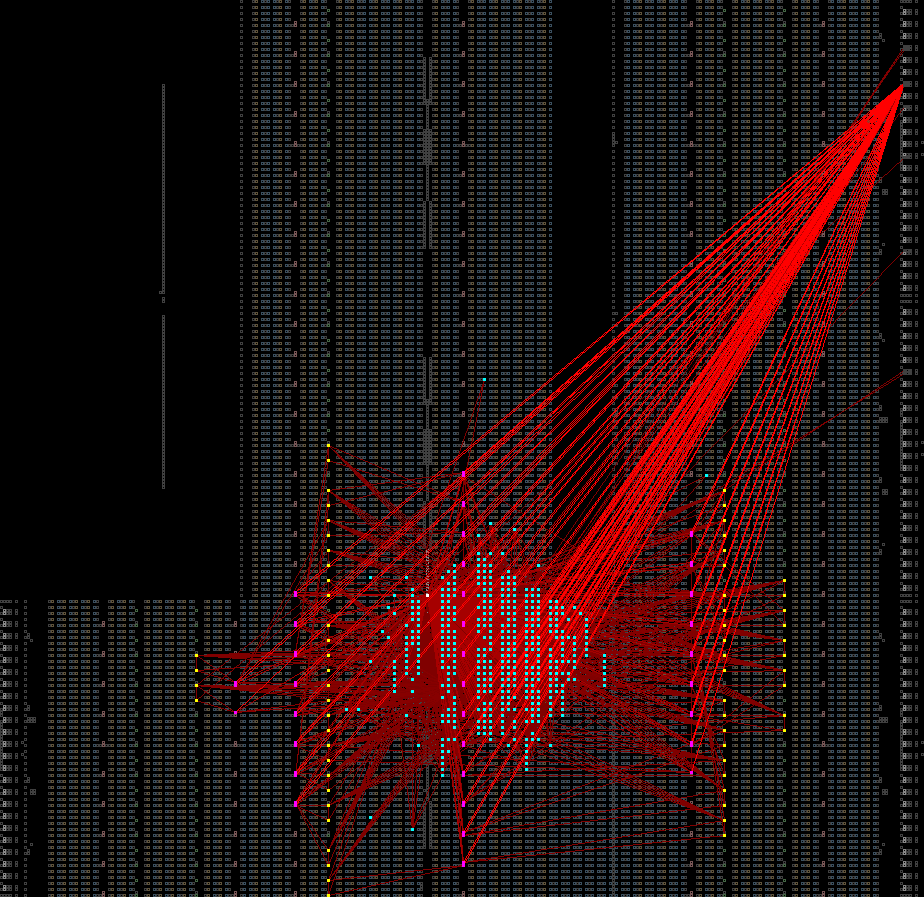
\includegraphics[valign=t, scale=0.13]{figures/results/PlacerGreedyRandom/00000299.png}
    \captionof{figure}{\texttt{PlacerGreedyRandom}}
    \label{fig:PGRSnapshots}
}

{
    \centering
    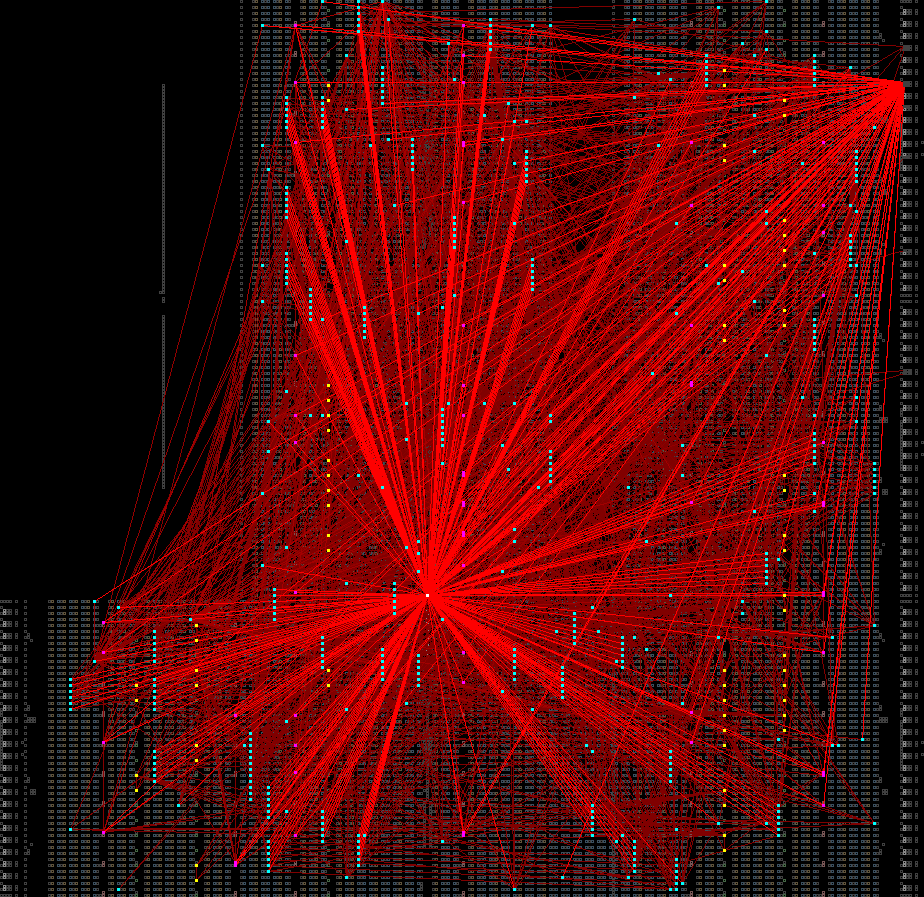
\includegraphics[valign=t, scale=0.13]{figures/results/PlacerGreedyMidpoint/random_placement.png}
    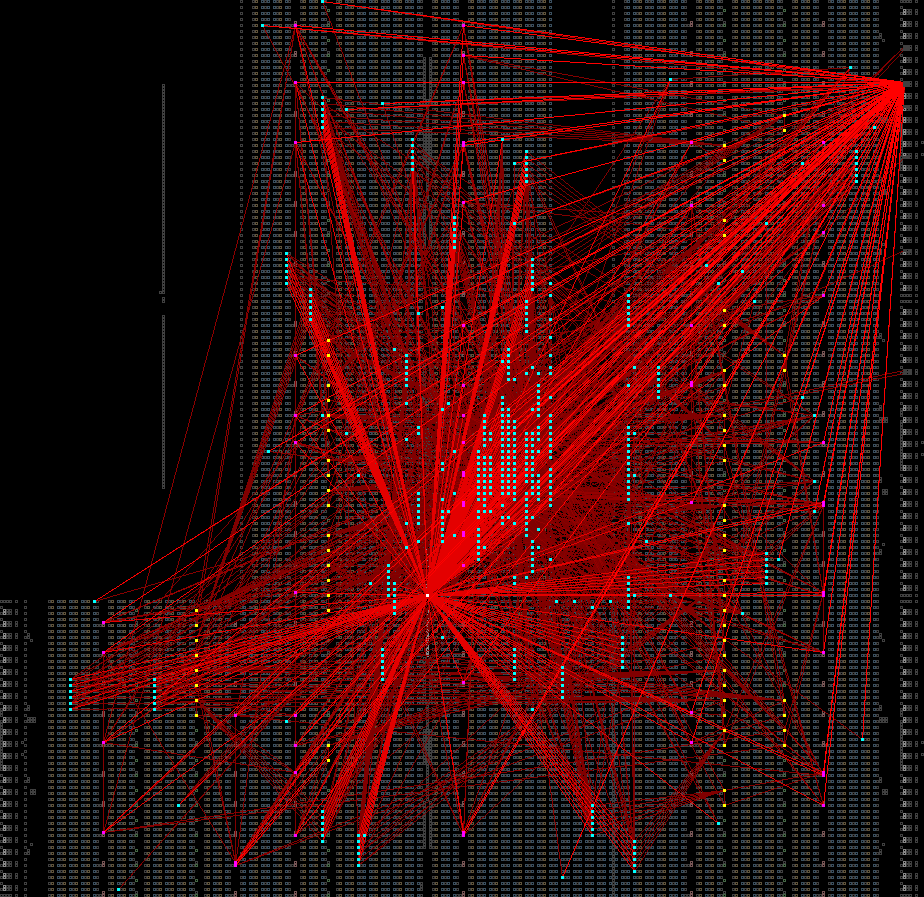
\includegraphics[valign=t, scale=0.13]{figures/results/PlacerGreedyMidpoint/00000010.png}
    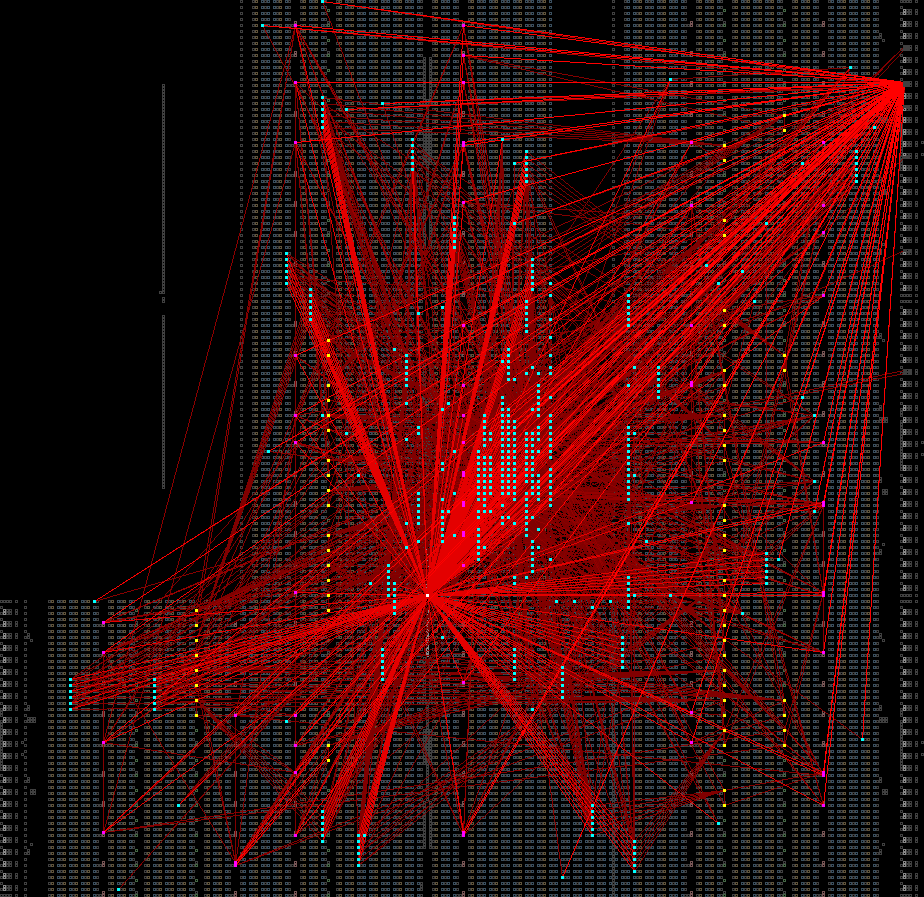
\includegraphics[valign=t, scale=0.13]{figures/results/PlacerGreedyMidpoint/00000100.png}
    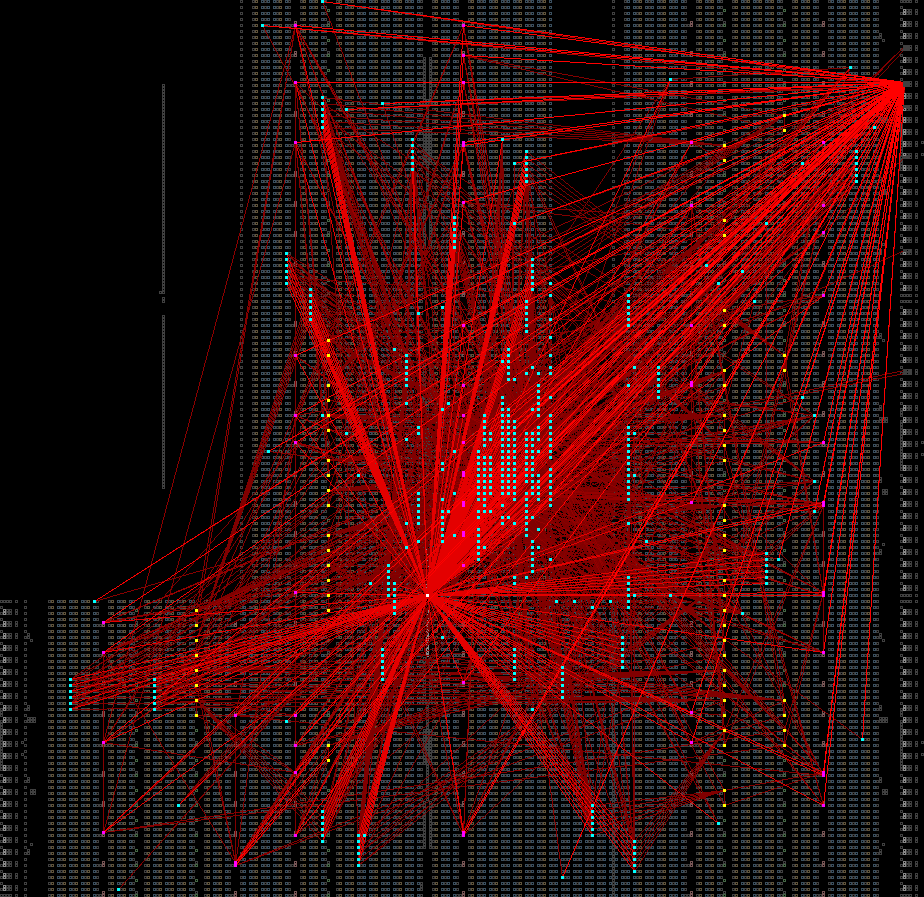
\includegraphics[valign=t, scale=0.13]{figures/results/PlacerGreedyMidpoint/00000299.png}
    \captionof{figure}{\texttt{PlacerGreedyMidpoint}}
    \label{fig:PGMSnapshots}
}

{
    \centering
    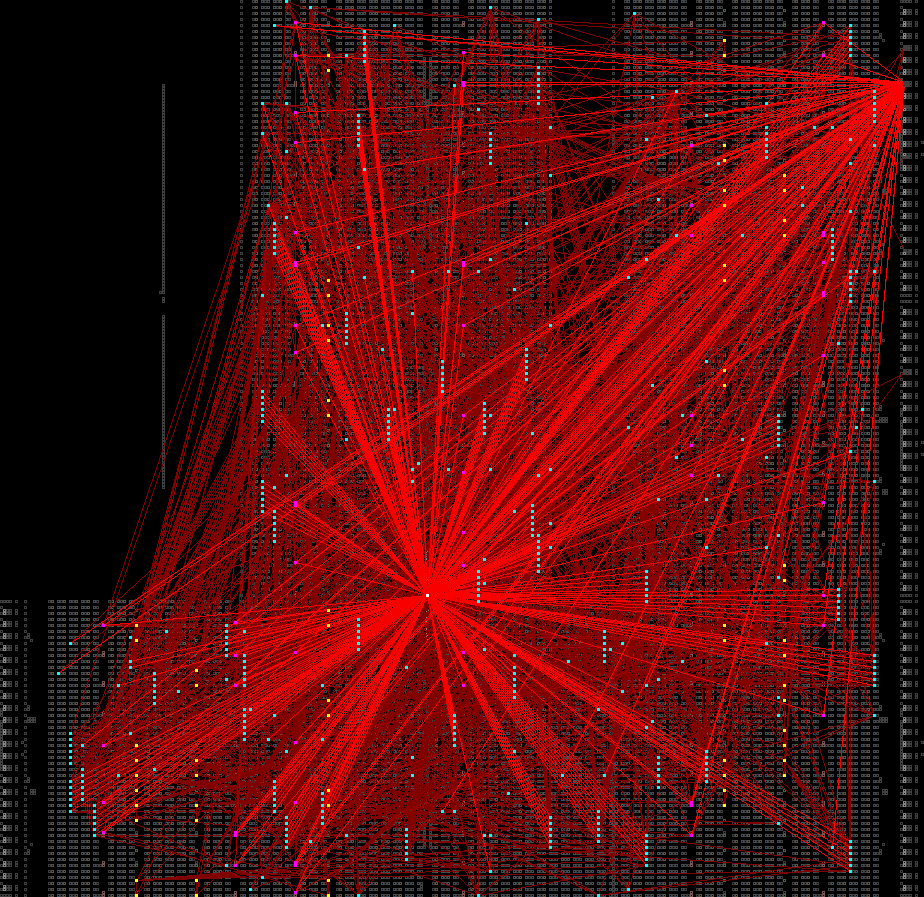
\includegraphics[valign=t, scale=0.13]{figures/results/PlacerAnnealRandom/random_placement.png}
    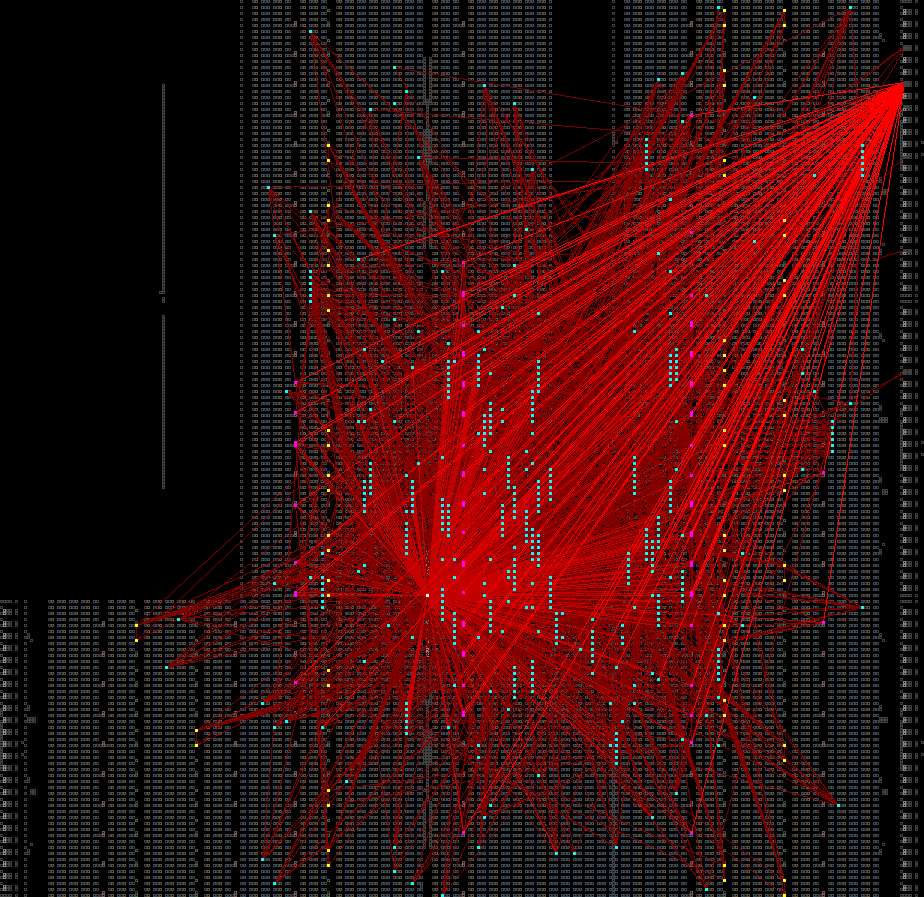
\includegraphics[valign=t, scale=0.13]{figures/results/PlacerAnnealRandom/00000010.png}
    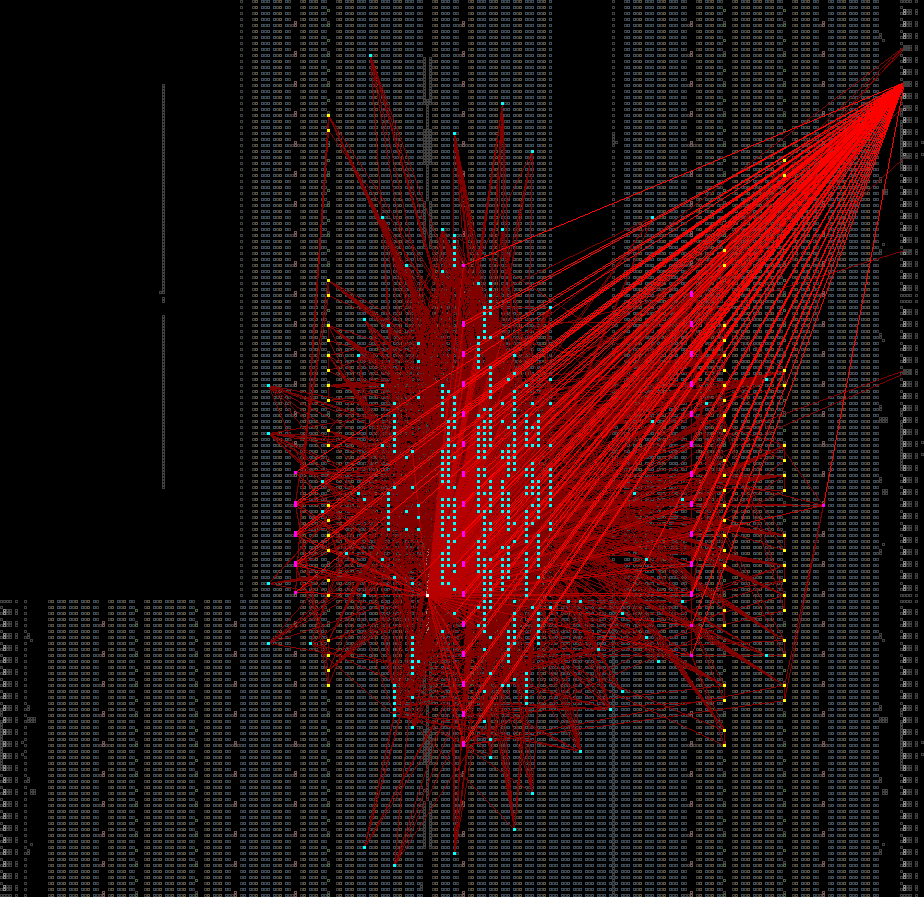
\includegraphics[valign=t, scale=0.13]{figures/results/PlacerAnnealRandom/00000100.png}
    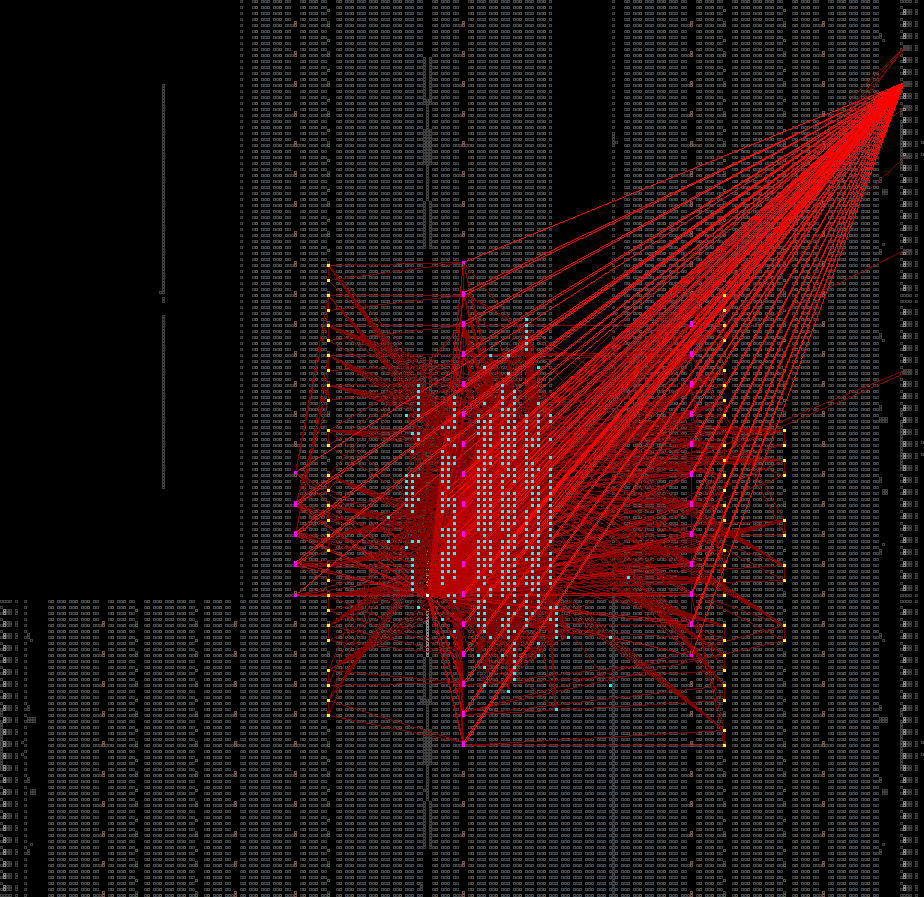
\includegraphics[valign=t, scale=0.13]{figures/results/PlacerAnnealRandom/00000299.png}
    \captionof{figure}{\texttt{PlacerAnnealRandom}}
    \label{fig:PARSnapshots}
}

{
    \centering
    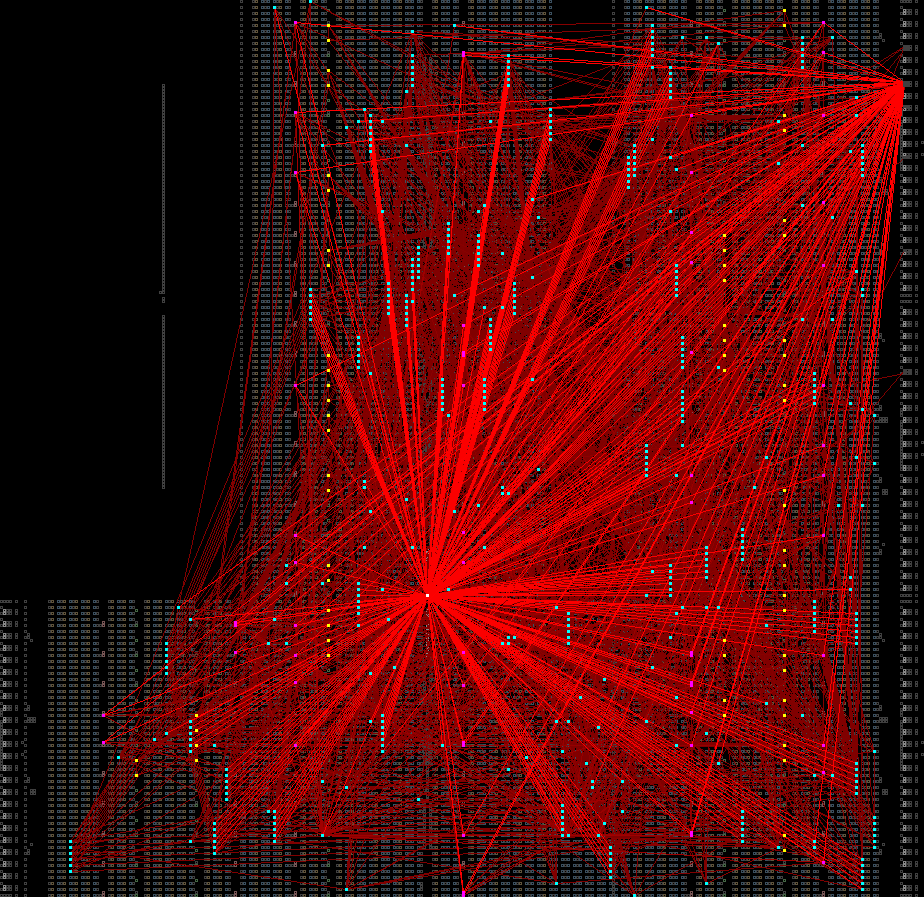
\includegraphics[valign=t, scale=0.13]{figures/results/PlacerAnnealMidpoint/random_placement.png}
    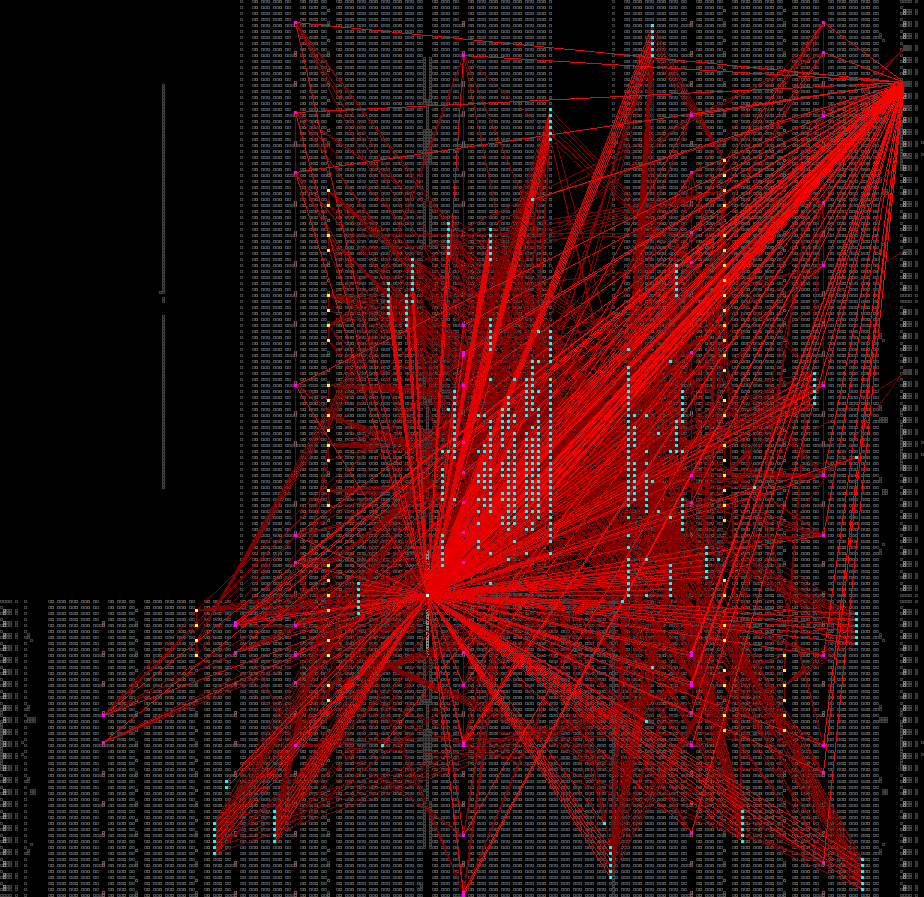
\includegraphics[valign=t, scale=0.13]{figures/results/PlacerAnnealMidpoint/00000010.png}
    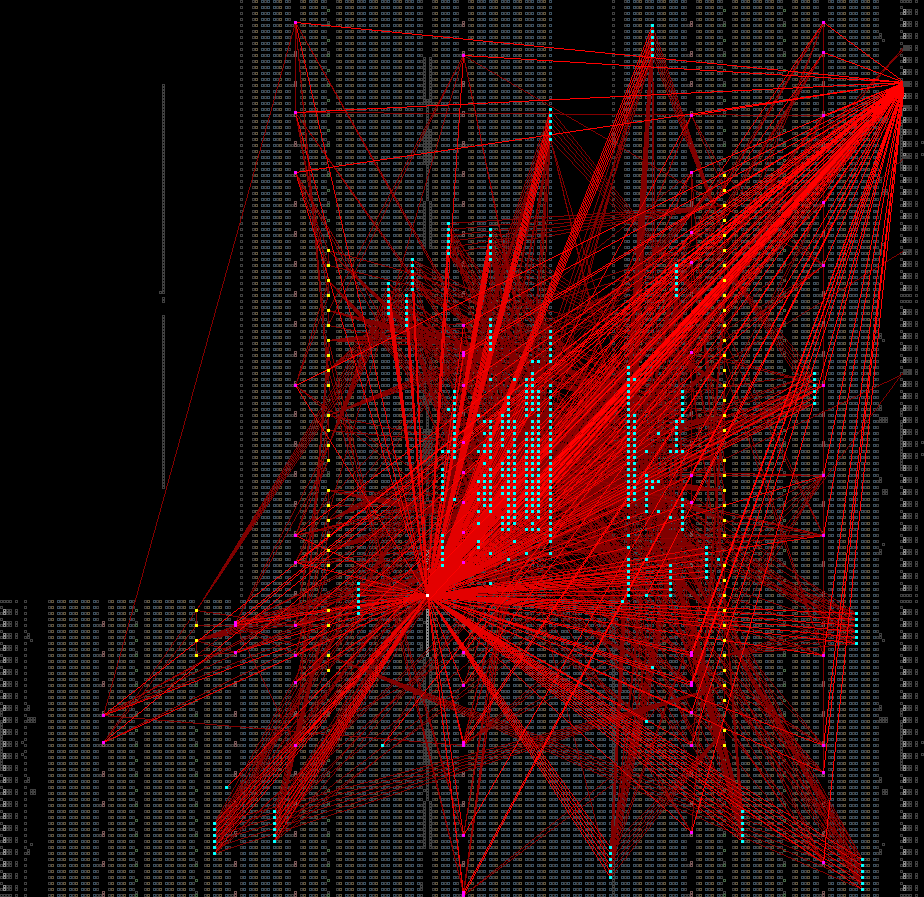
\includegraphics[valign=t, scale=0.13]{figures/results/PlacerAnnealMidpoint/00000100.png}
    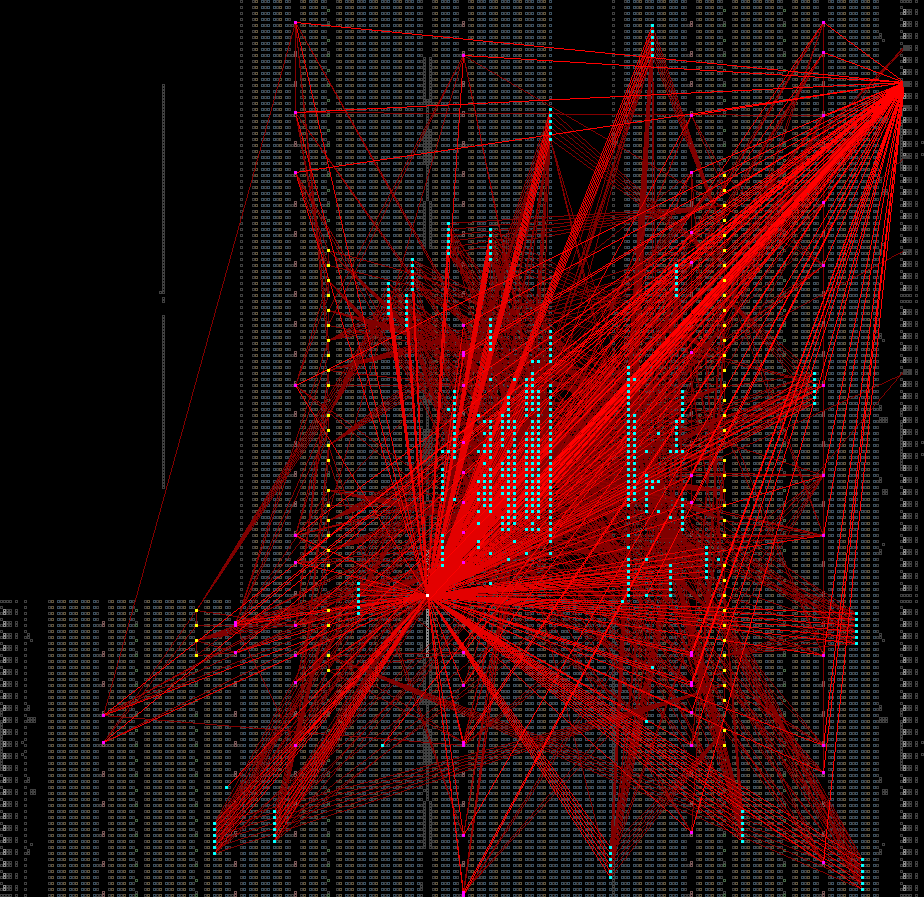
\includegraphics[valign=t, scale=0.13]{figures/results/PlacerAnnealMidpoint/00000299.png}
    \captionof{figure}{\texttt{PlacerAnnealMidpoint}}
    \label{fig:PAMSnapshots}
}

{
    \centering
    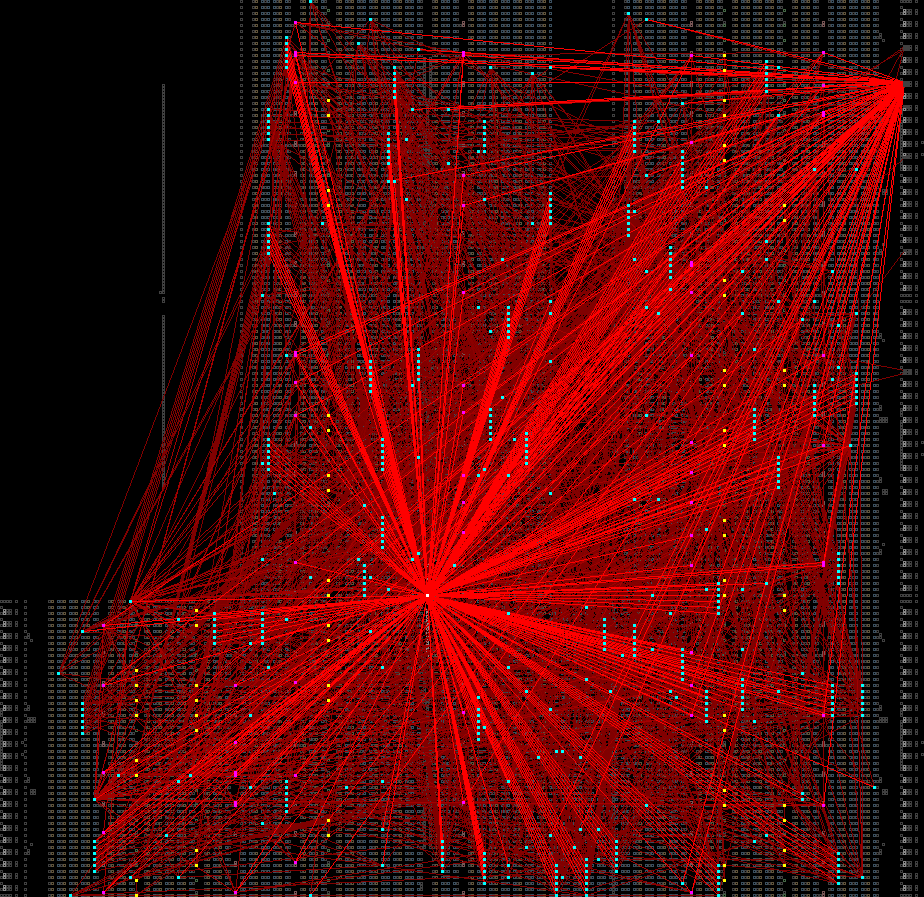
\includegraphics[valign=t, scale=0.13]{figures/results/PlacerAnnealHybrid/random_placement.png}
    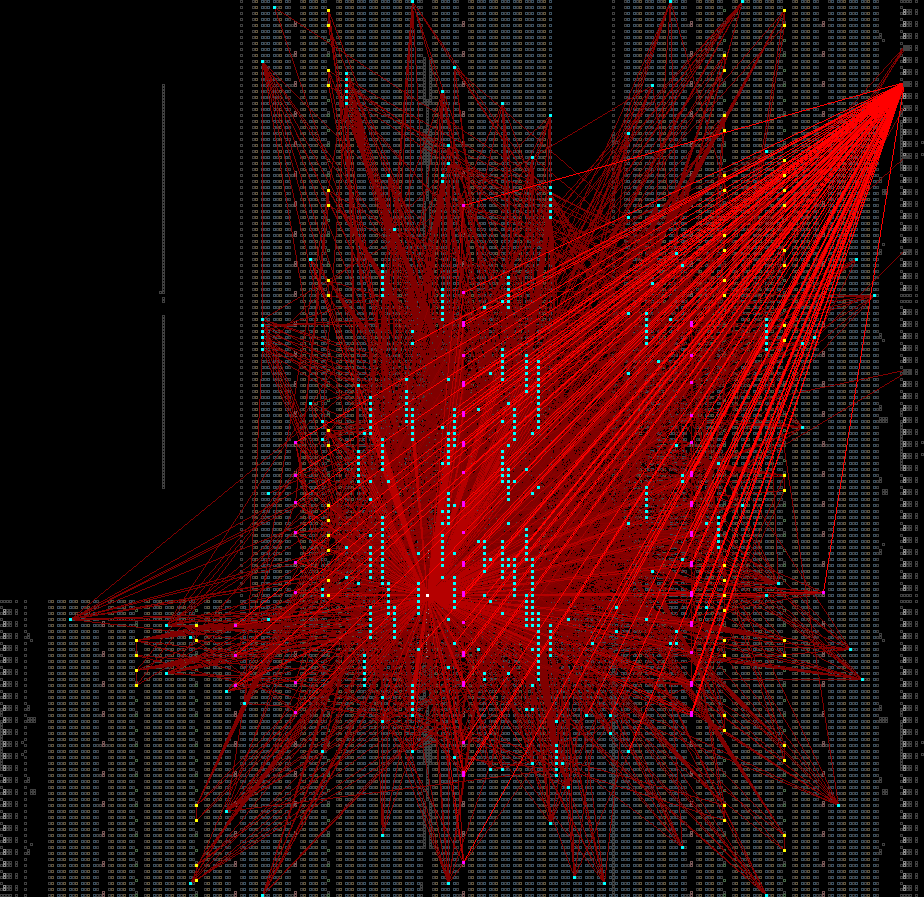
\includegraphics[valign=t, scale=0.13]{figures/results/PlacerAnnealHybrid/00000010.png}
    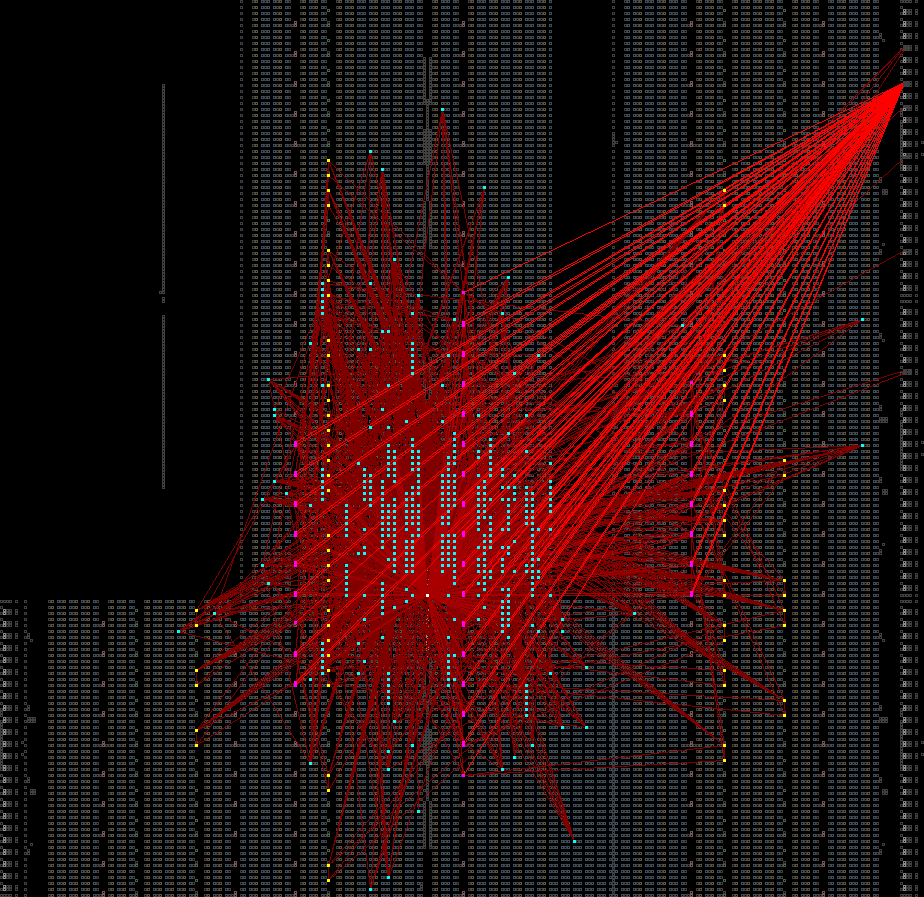
\includegraphics[valign=t, scale=0.13]{figures/results/PlacerAnnealHybrid/00000100.png}
    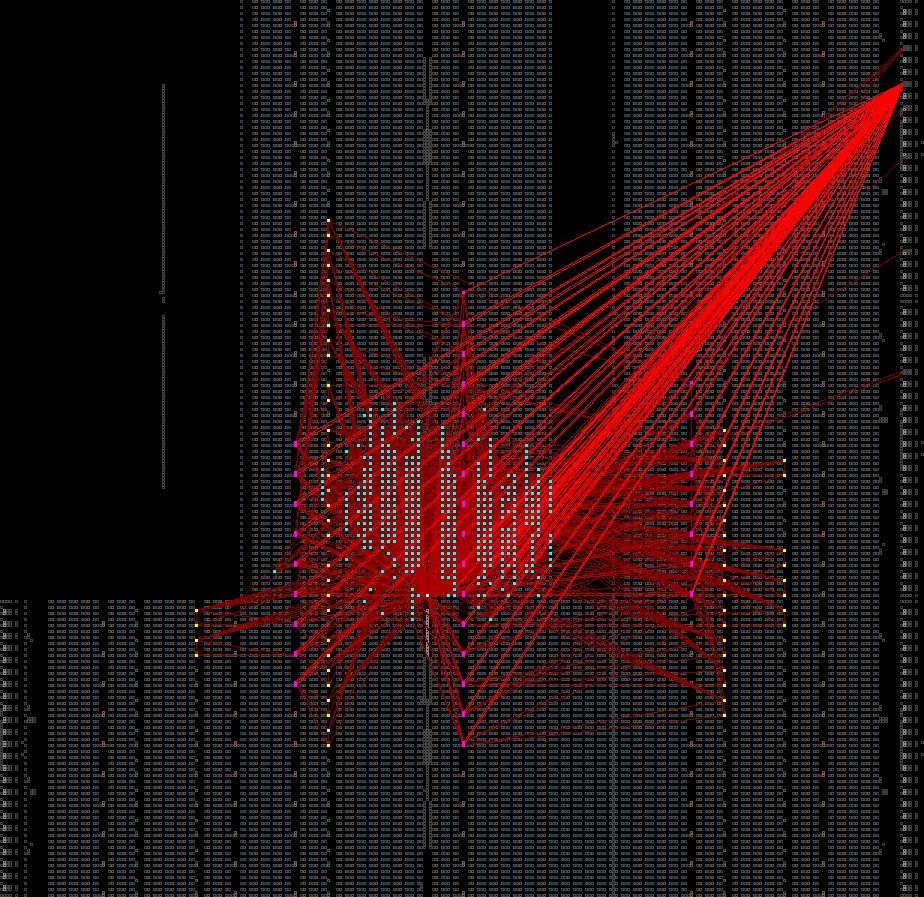
\includegraphics[valign=t, scale=0.13]{figures/results/PlacerAnnealHybrid/00000299.png}
    \captionof{figure}{\texttt{PlacerAnnealHybrid}}
    \label{fig:PAHSnapshots}
}

\begin{multicols}{2}
    In addition to variations on the basic SA algorithm, we also test various cooling schedules on the basic SA algorithm.
    Shown in figure \ref{fig:VaryCoolingSchedules} are the cost histories for various cooling schedules, grouped into three different initial temperatures \texttt{(5000, 10000, and 15000)}. 
    For each initial temperature group, we test five different cooling rates \texttt{(0.79, 0.84, 0.89, 0.94, and 0.99)}, with the darkness of each curve corresponding with a faster cooling rate.

\end{multicols}

{
    \centering
    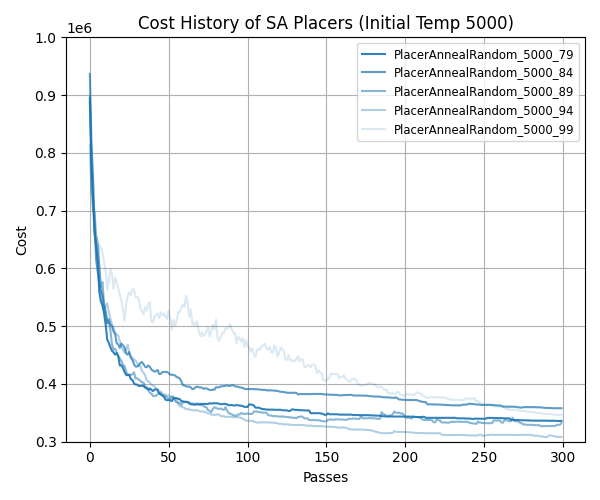
\includegraphics[valign=t, scale=0.55]{figures/results/cost_history_5000.png}
    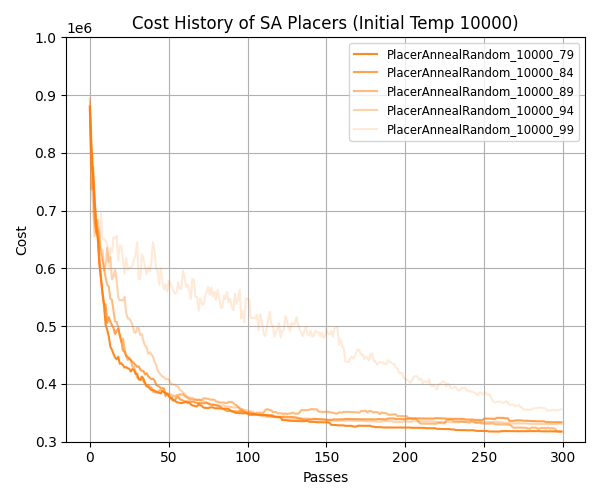
\includegraphics[valign=t, scale=0.55]{figures/results/cost_history_10000.png}
    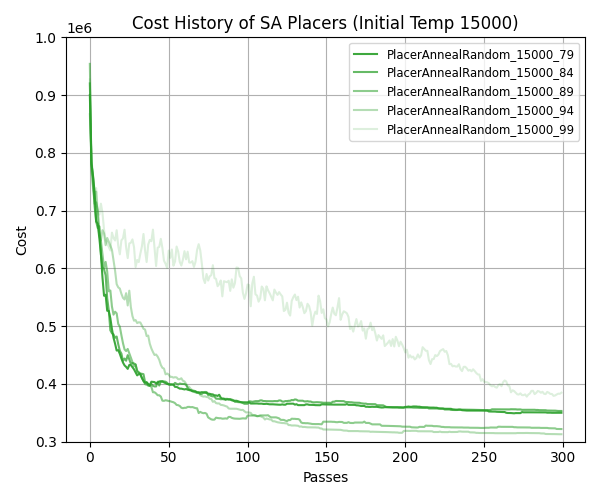
\includegraphics[valign=t, scale=0.55]{figures/results/cost_history_15000.png}
    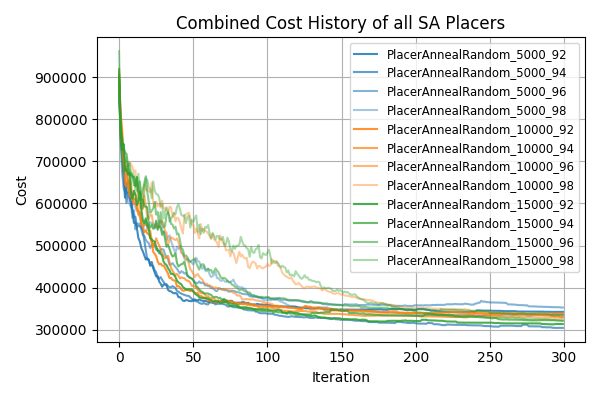
\includegraphics[valign=t, scale=0.55]{figures/results/combined_cost_history_cooling.png}
    \captionof{figure}{\texttt{PlacerAnnealRandom} with various cooling schedules.}
    \label{fig:VaryCoolingSchedules}
}

\begin{multicols}{2}


